\documentclass{beamer}

\input{../ts-glærur}

\title{FOR3R - Net}

\begin{document}
\begin{frame}
\titlepage
\end{frame}

\section{Um net}

\begin{frame}{Upprifjun úr síðasta tíma}
\begin{itemize}
 \item Hnútur (e. \emph{node}) inniheldur gögn og vísun í aðra hnúta
 \item Hægt er að raða hnútum upp í ýmsar gagnagrindur. Við höfum nefnt:
 \begin{itemize}
  \item Eintengda lista
  \item Tvítengda lista
  \item Tré
  \begin{itemize}
   \item Tvíleitartré
  \end{itemize}
 \end{itemize}
\end{itemize}
\end{frame}

\begin{frame}{Almenn net}
\begin{columns}
\column{0.5\textwidth}
\begin{itemize}
 \item Gagnagrindurnar sem við höfum skoðað hingað til og byggjast á hnútum hafa haft fastar reglur um hvernig hnútar þeirra mega tengjast saman 
 \begin{itemize}
  \item Þetta getur gert auðveldara að vinna með þau
 \end{itemize}
 \item Með því að leyfa almennari tengingar er hægt að tákna flóknari fyrirbrigði
\end{itemize}
\column{0.5\textwidth}
\begin{center}
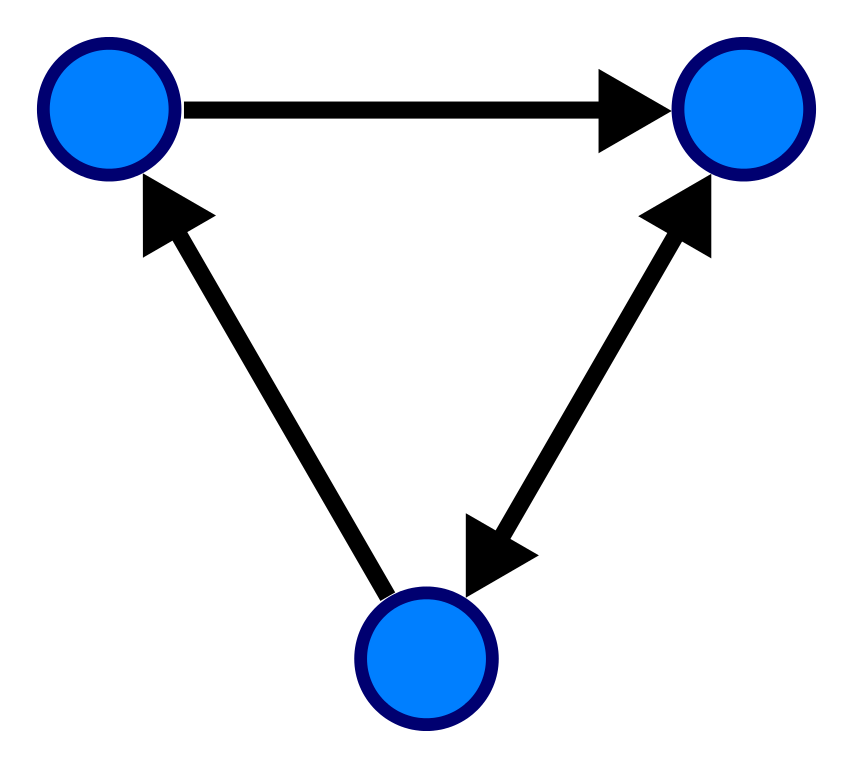
\includegraphics[width=\linewidth]{Pics/directed}

Stefnt net með 3 hnútum og 3 örvum 
\end{center}
\end{columns}
\end{frame}

\begin{frame}{Stefnd og óstefnd net}
\begin{columns}
\column{0.5\textwidth}
\begin{itemize}
 \item Hingað til höfum við verið að skoða hnúta þar sem einn hnútur ``bendir'' á annan
 \begin{itemize}
  \item M.ö.o. hver tenging á milli hnúta hefur \emph{stefnu}
  \item Algengt í forritun, vegna þess að það er auðveldara
 \end{itemize}
 \item Í stærðfræði er algengt að vinna með \emph{óstefnd} net, þar sem tengirnarnar eru jafnar í báðar áttir
\end{itemize}
\column{0.5\textwidth}
\begin{center}
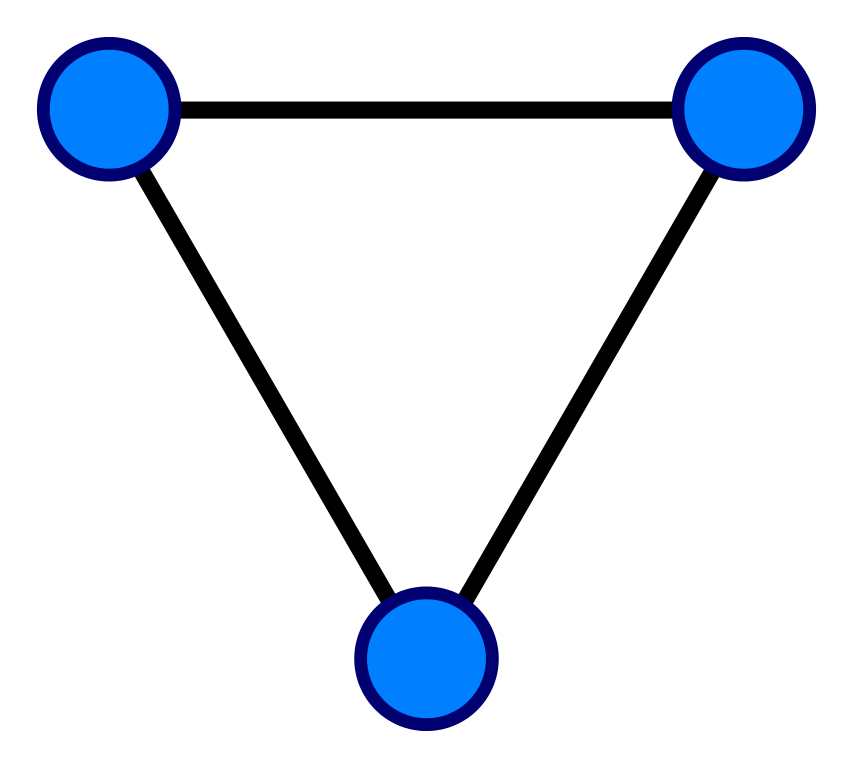
\includegraphics[width=\linewidth]{Pics/undirected}

Óstefnt net með 3 hnútum og 3 leggjum 
\end{center}
\end{columns}
\end{frame}

\begin{frame}{Meira um hugtök}
\begin{columns}
\column{0.5\textwidth}
Óstefnt net (e. \emph{undirected graph}) hefur leggi (e. \emph{edges}) á milli hnúta (e. \emph{nodes} eða \emph{vertices})
\begin{center}
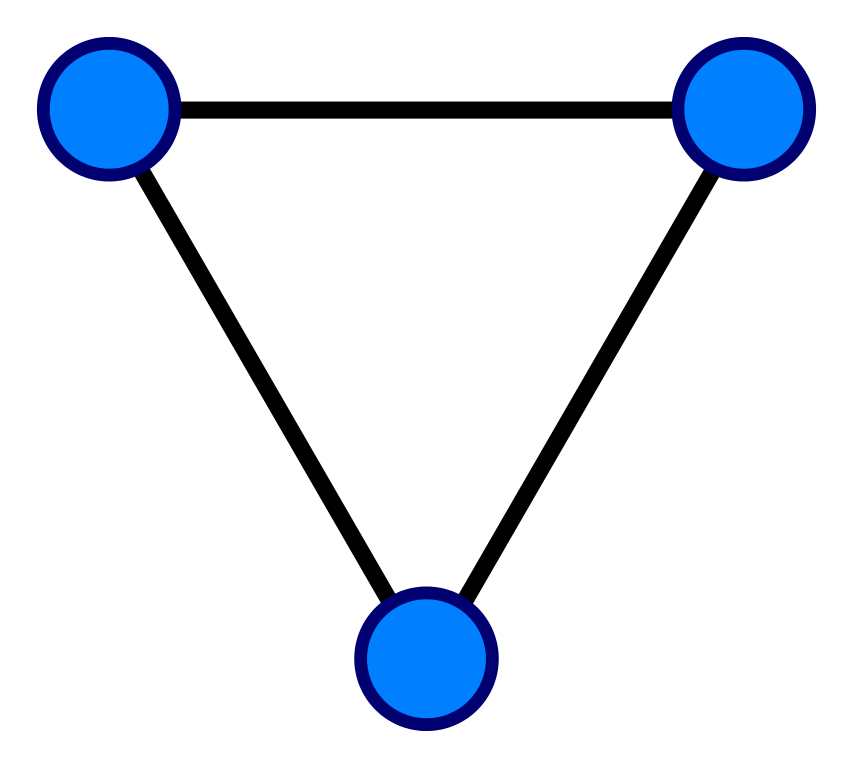
\includegraphics[width=0.7\linewidth]{Pics/undirected}
\end{center}
\column{0.5\textwidth}
Stefnt net eða örvanet (e. \emph{directed graph}) hefur örvar (e. \emph{directed edges}) á milli hnúta
\begin{center}
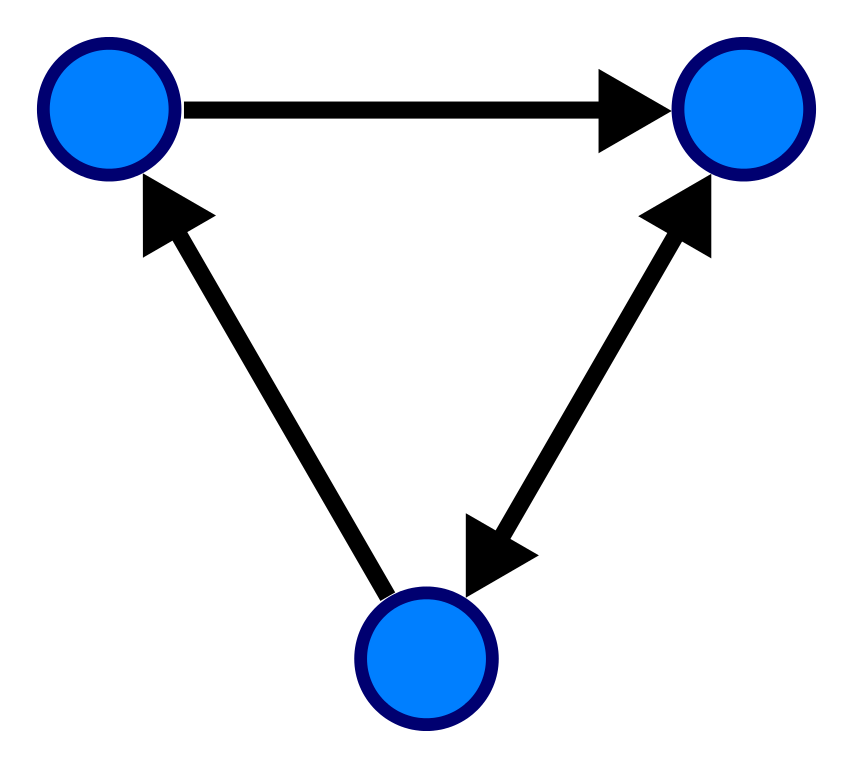
\includegraphics[width=0.7\linewidth]{Pics/directed}
\end{center}
\end{columns}
\end{frame}

\section{Hagnýtingarmöguleikar}

\begin{frame}{Hagnýting - Strætó}
\begin{itemize} 
 \item Getum notað net til að tákna strætókerfið
 \begin{itemize}
  \item Táknum allar strætóstoppistöðvar í Reykjavík með hnútum
  \item Táknum allar ferðir á milli stöðvanna með örvum
  \item Merkjum örvar með tölu sem táknar hversu langan tíma tekur að keyra leiðina
 \end{itemize}
 \item Getum þá spurt okkur:
 \begin{itemize}
  \item Er hægt að komast á milli allra stoppistöðva?
  \item Hver er fljótlegasta leiðin á milli tveggja stoppistöðva?
  \item Hvaða stöð hentar best sem aðalstoppistöð?
 \end{itemize}
\end{itemize}
\end{frame}

\begin{frame}{Hagnýting - rafmagnsdreifikerfi}
\begin{itemize}
 \item Notum net til að tákna rafmagnsdreifikerfi
 \begin{itemize}
  \item Táknum allar rafstöðvar í kerfinu með hnútum
  \item Táknum rafmagnslínu á milli þeirra með legg
  \item Merkjum alla leggi með burðargetu rafmagnslínunnar
 \end{itemize}
 \item Getum spurt okkur
 \begin{itemize}
  \item Hver er heildarburðargetan á milli tveggja stöðva?
  \item Hversu fáar rafmagnslínur komumst við upp með að leggja til að tengja allar stöðvarnar saman?
 \end{itemize}
\end{itemize}
\end{frame}

\section{Áhugaverðar staðreyndir}

\begin{frame}{Hversu vel þekkist fólk?}
\begin{itemize}
 \item Notum net til að tákna tengsl fólks
 \begin{itemize}
  \item Táknum fólk með hnútum
  \item Táknum það að fólk þekkist með legg á milli hnútanna
 \end{itemize}
 \item Getum spurt okkur
 \begin{itemize}
  \item Gildir að fjarlægð á milli hverra tveggja hnúta sé $\leq 6$?
  \item Hver þarf að meðaltali að leita styst til að tengjast hverjum sem er?
 \end{itemize}
\end{itemize}
\end{frame}


\begin{frame}{Litun}
Sönnun úr netafræði - einungis fjóra liti þarf til að lita tvívítt landakort (á flötum fleti eða hnetti)
\begin{columns}
\column{0.5\textwidth}
\begin{center}
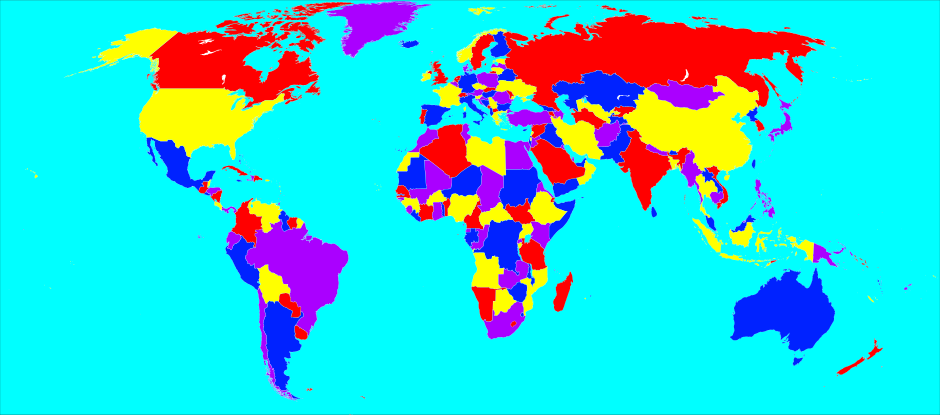
\includegraphics[width=\linewidth]{Pics/world-map-four-colors}
\end{center}
\column{0.5\textwidth}
\begin{center}
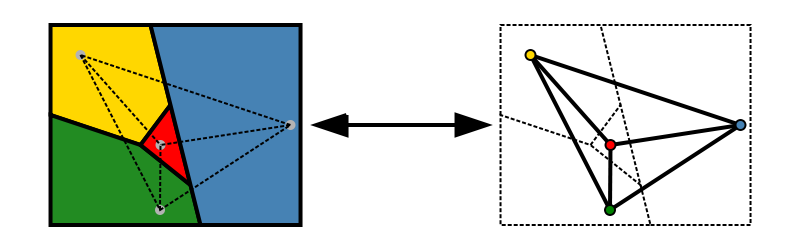
\includegraphics[width=\linewidth]{Pics/four-color}
\end{center}
\end{columns}
\vspace{0.5cm}
Fyrsta stóra stærðfræðisetningin sem sönnuð var með aðstoð tölvu
\end{frame}

\begin{frame}{Næst}
\begin{itemize}
 \item Í næstu viku skoðum við reiknirit sem svara sumum spurninganna sem settar voru fram
\end{itemize}

\end{frame}


\end{document}
